\documentclass{article}

\usepackage{listings}
\usepackage{enumitem}
\usepackage{amsmath}
\usepackage{svg}
\usepackage{hyperref}
\hypersetup{
    colorlinks=true,
    linkcolor=blue,
    filecolor=magenta,      
    urlcolor=cyan,
    pdftitle={Overleaf Example},
    pdfpagemode=FullScreen,
    }

\title{CA Lab: Lab 7}
\author{student: Dimitri Tabatadze}

\newcommand{\points}[1]{{\footnotesize{\color{red}\textit{#1 points}}}}

\definecolor{codegreen}{rgb}{0,0.6,0}
\definecolor{codegray}{rgb}{0.5,0.5,0.5}
\definecolor{codepurple}{rgb}{0.58,0,0.82}
\definecolor{backcolour}{rgb}{0.98,0.96,0.94}

\lstdefinestyle{mystyle}{
    backgroundcolor=\color{backcolour},   
    commentstyle=\color{codegreen},
    keywordstyle=\color{magenta},
    numberstyle=\tiny\color{codegray},
    stringstyle=\color{codepurple},
    basicstyle=\ttfamily\footnotesize,
    breakatwhitespace=false,         
    breaklines=true,                 
    captionpos=b,                    
    keepspaces=true,                 
    numbers=left,                    
    numbersep=5pt,                  
    showspaces=false,                
    showstringspaces=false,
    showtabs=false,                  
    tabsize=2
}

\lstset{style=mystyle}

\begin{document}
    \maketitle

    \section*{Task Description} 
    
    Write code for general purpose register file. MIPS processor has a register file that contains 32 registers. Each register is 32-bit long. Lab task is to design General Purpose Register File.

    Write Verilog code for 3 port general purpose register file. A port consists of an address and data input/output.

    \begin{enumerate}
        \item Give us the number of bits of \verb|addrA| and \verb|addrB|.
        \item Implement logic in your Verilog code that allows us to read values stored in registers.
        \item Implement logic in your Verilog code that allows us to update values stored in registers
        \item  In you code implement logic that makes sure that value stored in register \verb|$0| stays \verb|0| all the time.
        \item Write testbench for your design. Generate Waveforms and explain in your reports why do you think your design works correctly.
    \end{enumerate}

    \section*{Solution}

    \begin{enumerate}
        \item {
            The size of the addresses, \verb|addrA|, \verb|addrB| and \verb|addrC| should be \(\log_2(32) = 5\)
        }
        \item {
            The code that allows us to read the values stored at addresses \verb|addrA| and \verb|addrB|:

            \begin{lstlisting}[language=verilog]
// ...

always @(addrA)
    data_out_A <= register[addrA];

always @(addrB)
    data_out_B <= register[addrB];

// ...\end{lstlisting}
        }
        \item {
            The code that allows us to update the value stored at address \verb|addrC|:

            \begin{lstlisting}[language=verilog]
// ...

always @(posedge clk) begin
    if (write_enable) begin
        // ...

        register[addrC] <= data_in_C;

        // After the update, if the updated adresses are
        // supposed to be read, update the outputs accordingly.
        if (addrC == addrA)
            data_out_A <= data_in_C;
            
        if (addrC == addrB)
            data_out_B <= data_in_C;
        
        // ...
    end
end

// ...\end{lstlisting}
        }
        \item {
            The code that makes sure the value stored at address \verb|$0| never changes and stays \verb|0|:

            \begin{lstlisting}[language=verilog]
// ...

always @(posedge clk) begin
    if (write_enable) begin
        if (addrC != 0) begin // This check makes 
        // sure that only those addresses which 
        // are not 0 get updated.
            // ...
        end
    end
end

// ...\end{lstlisting}
        }
        \item {
            The whole testbench:

            \lstinputlisting[language=verilog]{gpr-tb.v}

            \begin{figure}[h] \caption{The timing diagram}
                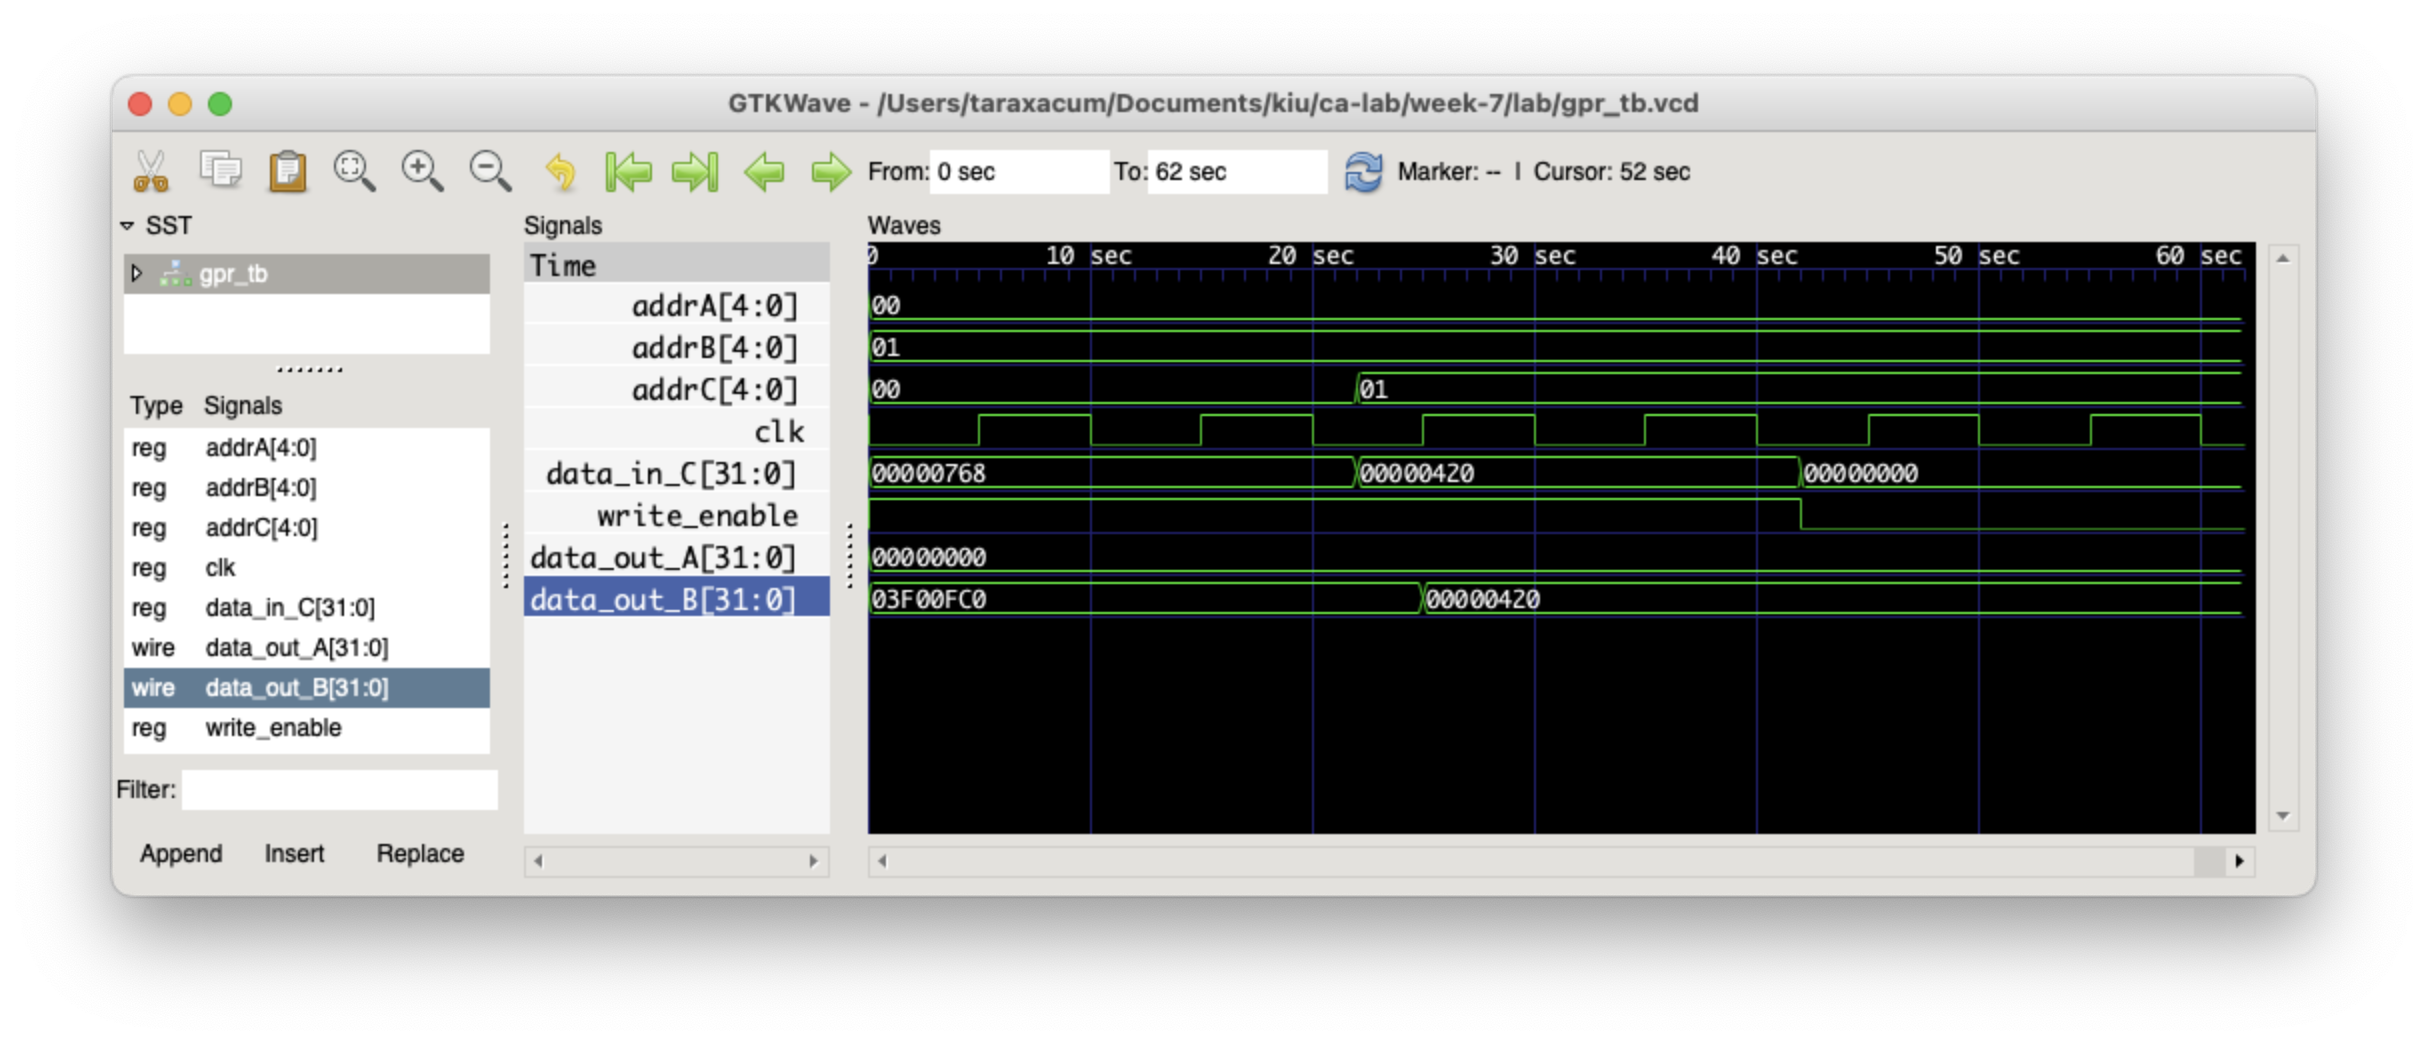
\includegraphics[width=12cm]{timing-diagram.png}
            \end{figure}
        }
    \end{enumerate}

    \section*{Conclusion}

    I think my implementation of the specified GPR is correct, because when given inputs, the outputs are correct (as far as I know).
    
    In case you want to see the full code for the GPR, here it is:
    
    \lstinputlisting[language=verilog]{gpr.v}

    and the contents of the corresponding "\verb|values.txt|":

    \lstinputlisting{values.txt}

    \section*{Reference}
    
    \begin{itemize}
        \item me.
    \end{itemize}

\end{document}